\section{Zustandsraumdarstellung (ZRD)}

\subsection{Zustrandsraumdarstellung von MIMO-Systemen}{153-154}

Der Vorteil der Zustandsraumdarstellung gegenüber der I/O-Beschreibung liegt darin, dass die internen Signale des Systems
(Zustandsvariablen) mitmodelliert werden. \\
Die ZRD kann aus dem Blockdiagramm abgeleitet werden. Umgekehrt kann aus der ZRD das Blockdiagramm
gezeichnet werden.

\smallskip

Die ZRD von MIMO-Systemen wird folgendermassen beschrieben:


\begin{center}
    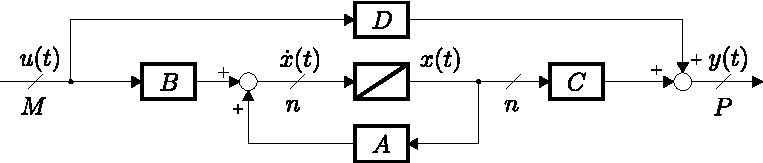
\includegraphics[width=0.75\columnwidth]{images/ZRD_blockdiagramm.pdf}
\end{center}

\begin{minipage}[c]{0.6\columnwidth}
        \fbox{\parbox{0.95\columnwidth}{
        $$ \dot{x}(t) = \bm{A} \cdot x(t) + \bm{B} \cdot u(t) $$
        $$ y(t) = \bm{C} \cdot x(t) + \bm{D} \cdot u(t) $$
    }}
\end{minipage}
\hfill
\begin{minipage}[c]{0.35\columnwidth}
    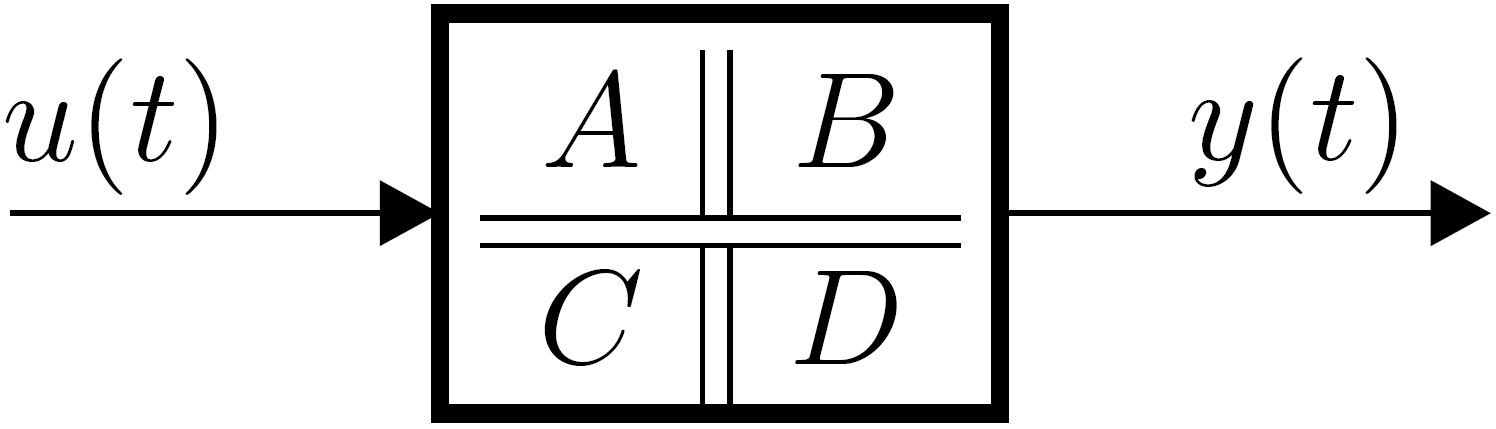
\includegraphics[width=\columnwidth]{images/ZRD_matrix_kompakt.png}
\end{minipage}


\begin{ctabular}{cll}
    \toprule
    $u(t) \in \mathbb{R}^{M}$               & Eingangsvektor    & fasst Eingangsgrössen in Vektor zusammen          \\
    \midrule
    $x(t)\in \mathbb{R}^{n}$                & Zustandsvektor    & fasst Zustände in Vektor zusammen                 \\
    \midrule
    $y(t)\in \mathbb{R}^{P}$                & Ausgangsvektor    & fasst Ausgangsgrössen in Vektor zusammen          \\
    \midrule
    $\bm{A} \in \mathbb{R}^{n \times n}$    & Systemmatrix      & beschreibt (Eigen-)Dynamik des Systems,           \\
                                            &                   & beschreibt \textbf{Stabilität} des Systems        \\
    \midrule
    $\bm{B} \in \mathbb{R}^{n \times M}$    & Eingangsmatrix    & beschreibt, wie der Eingang auf den               \\
                                            &                   & Zustandsvektor einwirken kann                     \\
    \midrule
    $\bm{C} \in \mathbb{R}^{P \times n}$    & Ausgangsmatrix    & beschreibt, welche Zustandsvariablen (oder        \\
                                            &                   & Linearkombinationen davon) \textbf{messbar} sind  \\
    \midrule
    $\bm{D} \in \mathbb{R}^{P \times M}$    & Durchgangsmatrix  & beschreibt direkte Kopplung zwischen Ein- und     \\
                                            &                   & Ausgang                                           \\
    \bottomrule
\end{ctabular}


\textbf{Hinweis:} Für Regelstrecken gilt aufgrund ihres Tiefpassverhaltens meist $\bm{D} = 0$


\subsubsection{ZRD für DGL der Ordnung $\bm{n}$}

\vspace{-0.2cm}

\begin{minipage}[c]{0.58\columnwidth}
    Für eine DGL der Ordnung $n$ werden die Zustände des Zustandsvektors $x$ jeweils so gewählt, dass der erste Zustand der 
    \textbf{unabgeleiteten} Variable entspricht und der letzte Zustand der $n-1$-ten Ableitung. \\
    \textrightarrow\ 'Kette' von Integratoren
\end{minipage}
\hfill
\begin{minipage}[c]{0.4\columnwidth}
    $$ x = \begin{bmatrix} x \\ \dot{x} \\ \vdots \\ x^{(n-1)}\end{bmatrix}
    \quad \Rightarrow\
    \dot{x} = \begin{bmatrix} \dot{x} \\ \ddot{x} \\ \vdots \\ x^{(n)}\end{bmatrix} $$
\end{minipage}


\subsection{Zustrandsraumdarstellung von SISO-Systemen}{154}

\begin{minipage}[c]{0.5\columnwidth}
        \fbox{\parbox{0.95\columnwidth}{
        $$ \dot{x}(t) = \bm{A} \cdot x(t) + b \cdot u(t) $$
        $$ y(t) = c \cdot x(t) + d \cdot u(t) $$
    }}
\end{minipage}
\hfill
\begin{minipage}[c]{0.45\columnwidth}
    Wegen $M = P =1$ werden die Matritzen $\bm{B}$ und $\bm{C}$ zu Vektoren. \\
    $\bm{D}$ wird zu einem Skalar.
\end{minipage}


\subsection{Verfahren mit ZRD -- Übersicht}

Zum Thema ZRD werden die folgenden Verfahren genauer betrachtet, bevor diese auf die Regelungstechnik angewendet werden.

\smallskip

\begin{tabular}{ll}
    \tabitem ZRD aus Modellierung nach physikalischen Prinzipien                & \ref{ZRD via physikalischer Modellbildung}            \\
    \tabitem Lineariserung einer nichtlinearen ZRD                              & \ref{Linearisierung einer ZRD}                        \\
    \tabitem ZRD aus einer UTF oder DGL bestimmen                               & \ref{Zustandsraumdarstellung aus einer UTF oder DGL}  \\
    \tabitem Herauslesen der ZRD aus einem Blockdiagramm                        & \ref{Zustandsraumdarstellung aus Blockdiagramm}       \\
    \tabitem Aggregation von Teilsystem (Serie-, Parallel-, Kreisschaltung)     & \ref{Aggregation von Teilsystemen}                    \\
    \tabitem Ähnlichkeitstransformation durch andere Wahl des Zustandsvektors   & \ref{Ähnlichkeitstransformation}                      \\
\end{tabular}


\subsection{ZRD via physikalischer Modellbildung}
\label{ZRD via physikalischer Modellbildung}

Aus einem physikalischen System werden die Eingang- und Ausgangssignale, sowie die Zustände bestimmt. Diese werden mathematisch / physikalisch
beschrieben und als ZRD dargestellt.

\subsubsection{Vorgehen -- Herleitung eines ZRD-Modells}

\begin{enumerate}
    \item Anzahl Speicher (Integratoren) bestimmen
    \item Wahl der Zustandsgrössen
    \item Beschreibung der \textbf{Änderung} (Ableitungen) der Zustandsgrössen als Gleichungen
    \item Substitution der 'nicht-Zustandsgrössen' mittls algebraischer Gleichungen
    \item Bilden der Zustands- und Ausgangsgleichungen
    \item Darstellung in Matrix-Notation
\end{enumerate}



\example{ZRD eines RLC-Systems}{155-156}

\begin{minipage}[t]{0.3\columnwidth}
    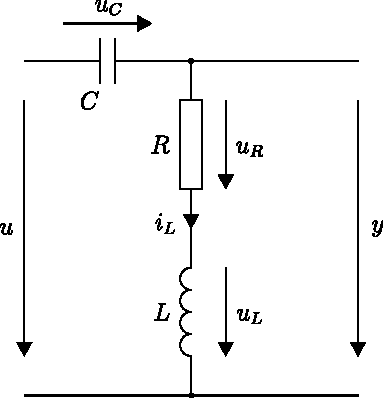
\includegraphics[width=\columnwidth, align=t]{images/ZRD_beispiel_schaltkreis.pdf}
\end{minipage}
\hfill
\begin{minipage}[t]{0.67\columnwidth}
    \begin{outline}
        \1 SISO-System mit zwei Speichern \textrightarrow\ zwei Zustände
            \2 Kondensator \textrightarrow\ $u_C$ (bzw. Ladung)
            \2 Spule \textrightarrow\ $i_L$
    \end{outline}

    \medskip
    
    Somit ergibt sich folgender Zustandsvektor
    $$ x(t)   = \begin{bmatrix} x_1 \\ x_2 \end{bmatrix}
                    = \begin{bmatrix} u_C \\ i_L \end{bmatrix} $$

                
    Die Netzwerkgleichungen ergeben sich aus dem Schema.
\end{minipage}

\smallskip

\renewcommand{\arraystretch}{1.5}
\begin{tabular}{lll}
    Knoten:             & $C \cdot \dot{u}_C = i_C = i_L$                               & \textrightarrow\ $\dot{u}_C = \frac{i_L}{C}$                                          \\
    Eingangsmasche:     & $L \cdot \dot{i}_L = u - u_C - u_R = u - u_C - R \cdot i_L$   & \textrightarrow\ $\dot{i}_L = \frac{u}{L} - \frac{u_C}{L} - \frac{R}{L} \cdot i_L$    \\
    Äussere Masche:     & $u = u_C + y$                                                 & \textrightarrow\ $y = u - u_C$                                                        \\
\end{tabular}
\renewcommand{\arraystretch}{1}

\medskip

Die drei (linearen) Gleichungen rechts können direkt in die ZRD gebracht werden, indem sie in Matritzen geschrieben werden.

\vspace{-0.4cm}

\begin{align*}
    \dot{x}(t)  &= \begin{bmatrix} \dot{u}_C \\ \dot{i}_L \end{bmatrix}
                 = \begin{bmatrix} 0 & \frac{1}{C} \\ - \frac{1}{L} & - \frac{R}{L} \end{bmatrix} \cdot \overbrace{ \begin{bmatrix} u_C \\ i_L \end{bmatrix} }^{x(t)}
                 + \begin{bmatrix} 0 \\ \frac{1}{L} \end{bmatrix} \cdot u(t)\\
    y(t)        &= \begin{bmatrix} -1 & 0 \end{bmatrix} \cdot  \underbrace{ \begin{bmatrix} u_C \\ i_L \end{bmatrix} }_{x(t)} + 1 \cdot u(t)
\end{align*}

\vspace{-0.3cm}

%-----------------------------------------------------------------------------------------------------------------------------------
\example{Feder-Masse-System}

Kraftbilanz:

\[
m\ddot p = F_u-kp
\]

Zustände:

\[
x_1=p,
\qquad
x_2=\dot p
\]

ZRD:

\[
\dot x=
\begin{bmatrix}
0 & 1\\
-\frac{k}{m} & 0
\end{bmatrix}
x+
\begin{bmatrix}
0\\
\frac{1}{m}
\end{bmatrix}
u
\]

\[
y=
\begin{bmatrix}
1 & 0
\end{bmatrix}
x
\]
%------------------------------------------------------------------------------------------------------------------------------------

\subsection{Linearisierung einer ZRD}{168}
\label{Linearisierung einer ZRD}

Die Linearisierung eines Systems erfolgt üblicherweise in einem Arbeitspunkt, damit relativ einfach ein Regler für diesem Arbeitspunkt 
entwickelt werden kann.

\smallskip

Wenn ein System in einem Arbeitspunkt linearisiert wird, has das zur Folge,

\begin{enumerate}
    \item dass das Verhalten des nichtlinearen Systems in einer 'kleineren' Umgebung um den Arbeitspunkt erhalten bleibt.
    \item dass das linearisierte System dieses Verhalten, entsprechend 'gestreckt', im ganzen Zustandsraum zeigt.
\end{enumerate}


\subsubsection{Linearisierte ZRD}

Die linearisierte ZRD für ein nichtlineares System in einem Arbeitspunkt mit $f(x_0, u_0) = 0$ und $y_0 = g(x_0, u_0)$ kann gewonnen werden, indem 
die 'Deltas' gebildet werden. \\
(Die $\Delta$-Symbole werden in der Notation jedoch oft weggelassen.)

\begin{ctabular}{llll}
    Zustandsgleichung(en)   & $\dot{x} = f(x, u)$ & \textrightarrow\  & $\Delta \dot{x} = A \cdot \Delta x + B \cdot \Delta u$    \\
    Ausgangsgleichung(en)   & $y = g(x, u)$       & \textrightarrow\  & $ \Delta y = C \cdot \Delta x + D \cdot \Delta u $
\end{ctabular}

Dazu werden die folgenden Jacobi-Matritzen benötigt, welche im Arbeitspunkt $(x_0, u_0)$ ausgewertet werden.

$$ 
    A =
    \left. \begin{bmatrix}
        \frac{\partial f_1}{\partial x_1} & \cdots & \frac{\partial f_1}{\partial x_n} \\
        \vdots & \ddots & \vdots \\
        \frac{\partial f_n}{\partial x_1} & \cdots & \frac{\partial f_n}{\partial x_n}
    \end{bmatrix} \right|_{x_0, u_0}
    \quad
    B =
    \left. \begin{bmatrix}
        \frac{\partial f_1}{\partial u_1} & \cdots & \frac{\partial f_1}{\partial u_M} \\
        \vdots & \ddots & \vdots \\
        \frac{\partial f_n}{\partial u_1} & \cdots & \frac{\partial f_n}{\partial u_M}
    \end{bmatrix} \right|_{x_0, u_0}
$$

$$
    C =
    \left. \begin{bmatrix}
        \frac{\partial g_1}{\partial x_1} & \cdots & \frac{\partial g_1}{\partial x_n} \\
        \vdots & \ddots & \vdots \\
        \frac{\partial g_P}{\partial x_1} & \cdots & \frac{\partial g_P}{\partial x_n}
    \end{bmatrix} \right|_{x_0, u_0}
    \quad
    D =
    \left. \begin{bmatrix}
        \frac{\partial g_1}{\partial u_1} & \cdots & \frac{\partial g_1}{\partial u_M} \\
        \vdots & \ddots & \vdots \\
        \frac{\partial g_P}{\partial u_1} & \cdots & \frac{\partial g_P}{\partial u_M}
    \end{bmatrix} \right|_{x_0, u_0}
$$


\subsubsection{Vorgehen -- Linearisierung}

\begin{enumerate}
    \item Statischen Arbeitspunkt $(u_0, \, y_0)$ festlegen \\
        \textbf{Im AP sind alle Ableitungen $\bm{0}$} \textrightarrow\ $\dot{x} = f(x, u) \overset{!}{=} 0$
    \item ZRD durch Berechnung der Jacobi-Matzitzen linearisieren (Auswertung im AP)
\end{enumerate}
%=============================================================================================================================
\para{Arbeitspunkt}

Im Arbeitspunkt gilt:

\[
\dot{x}_0=f(x_0,u_0)=0
\]

\textrightarrow\ Alle Ableitungen auf Null setzen und nach $x_0$ bzw. $u_0$ auflösen.
%===============================================================================================================================

\subsection{Zustandsraumdarstellung aus UTF oder DGL}{169-170}
\label{Zustandsraumdarstellung aus einer UTF oder DGL}

Für die folgenden Betrachtungen wird die UTF in einer Form betrachtet, in der ein allfälliger Proportionalteil durch den Term $d$
repräsentiert wird.

$$ G(s) = \frac{Y(s)}{U(s)} = d + \frac{b_m s^m + b_{m-1} s^{m-1} + \ldots + b_1 s + b_0}{s^n + a_{n-1} s^{n-1} + \ldots + a_1 s + a_0} \qquad (m < n)$$


Ein entsprechendes Blockdiagramm in \textbf{Regelungsnormalform} hat folgende Struktur:

\begin{center}
    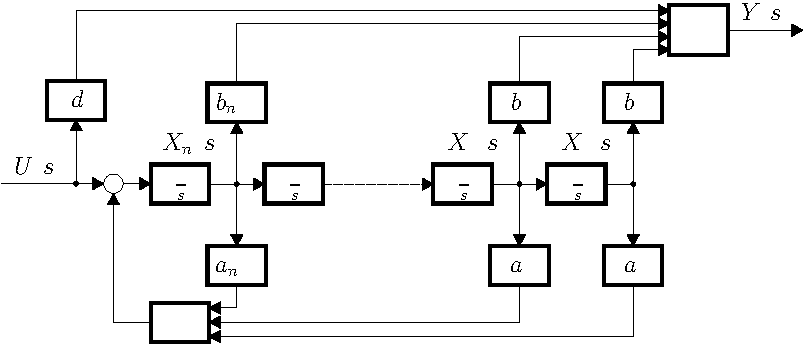
\includegraphics[width=0.75\columnwidth]{images/ZRD_regelungsnormalform.pdf}
\end{center}

In den Zeitbereich transformiert ergibt sich folgende Zustandsraumdarstellung:

$$
\overbrace{
\begin{bmatrix}
    \dot{x}_1 \\ \dot{x}_2 \\ \vdots \\ \dot{x}_{n-1} \\ \dot{x}_n
\end{bmatrix}
}^{\dot{x}}
=
\overbrace{
\begin{bmatrix}
    0       & 1         & 0         & \cdots    & 0         \\
    0       & 0         & 1         & \ddots    & \vdots    \\
    \vdots  & \vdots    & \ddots    & \ddots    & 0         \\
    0       & 0         & \cdots    & 0         & 1         \\
    -a_0    & -a_1      & \cdots    & -a_{n-2}  & -a_{n-1}
\end{bmatrix}
}^{A}
\cdot 
\overbrace{
\begin{bmatrix}
    x_1 \\ x_2 \\ \vdots \\ x_{n-1} \\ x_n
\end{bmatrix}
}^{x}
+
\overbrace{
\begin{bmatrix}
    0 \\ 0 \\ \vdots \\ 0 \\ 1
\end{bmatrix}
}^{b} \cdot  u
$$

$$
y =
\underbrace{
\begin{bmatrix}
    b_0 & b_1 & \cdots & b_{n-2} & b_{n-1}
\end{bmatrix}
}_{c}
\begin{bmatrix}
    x_1 \\ x_2 \\ \vdots \\ x_{n-1} \\ x_n
\end{bmatrix}
+ d \cdot u
$$


\subsubsection{Eindeutigkeit}

\begin{outline}
    \1 Aus einer UTF eine Zustandsraumdarstellung zu gewinnen ist \textbf{nicht eindeutig}. Auf triviale Art lassen sich alternative Formen
        produzieren (z.B. Zustandsvariablen anders nummerieren)
    \1 Aus einer ZRD die UTF zu gewinnen ist \textbf{eindeutig}
\end{outline}


\subsection{ZRD im Bildbereich}



\begin{minipage}[c]{0.5\columnwidth}
    Die ZRD existiert auch im Bildbereich und hat die Form:
\end{minipage}
\hfill
\begin{minipage}[c]{0.45\columnwidth}
        \fbox{\parbox{0.9\columnwidth}{
            \vspace{-0.3cm}
            \begin{align*}
                s X(s)  &= \bm{A} \cdot X(s) + \bm{B} \cdot U(s) + x(0) \\
                Y(s)    &= \bm{C} \cdot X(s) + \bm{D} \cdot U(s)
            \end{align*}
            \vspace{-0.5cm}
    }}
\end{minipage}


\subsubsection{UTF aus ZRD (Bildbereich)}

\vspace{-0.3cm}

\begin{minipage}[c]{0.44\columnwidth}
    Die UTF $G(s)$ kann durch den Zusammenhang rechts gewonnen werden.

    \smallskip

    \textbf{Hinweis:} In der UTF $G(s)$ kommen keine (statischen) Zustände $x_0$ mehr vor.
\end{minipage}
\hfill
\begin{minipage}[c]{0.52\columnwidth}
    \begin{align*}
        Y(s)    &= \bm{C} \cdot \overbrace{(s \bm{I} - \bm{A})^{-1} \cdot \bm{B} \cdot U(s)}^{X(s)} + \bm{D} \cdot U(s)  \\
                &= \underbrace{\left[ \bm{C} \cdot (s \bm{I} - \bm{A})^{-1} \cdot \bm{B} + \bm{D} \right]}_{G(s)} \cdot U(s)
    \end{align*}
\end{minipage}


\subsection{Zustandsraumdarstellung aus Blockdiagramm}{171}
\label{Zustandsraumdarstellung aus Blockdiagramm}

Mittels folgendem Vorgehen kann die ZRD aus dem Blockdiagrmam bestimmt werden:

\smallskip
\begin{enumerate}
    \item Eingangs- und Ausgangssignale bestimmen
    \item Zustandsvektor bilden, indem alle Speicher aufgelistet werden \\
        \textrightarrow\ Länge des Zustandsvektors entspricht Systemordnung \\
        \textrightarrow\ entspricht Summe der Ordnung der Teilsysteme
    \item Gleichung $\dot{x} = f(x, u)$ bilden, indem alle Intergratoreingänge $(=\dot{x}_i)$ 'zurückverfolgt' werden,
        bis deren Abhängigkeit von Eingangssignalen \& Zustandsvariablen definiert ist
    \item Gleichung $y = g(x, u)$ bilden, indem Ausgangssignale $(=y_i)$ 'zurückverfolgt' werden, bis deren Abhängigkeit von 
        Eingangssignalen \& Zustandsvariablen definiert ist
    \item Bei linearen Systemen: Gleichungen $f$ und $g$ mit Matritzen $\bm{A}, \, \bm{B}, \, \bm{C}$ und $\bm{D}$ formulieren
\end{enumerate}

\vspace{-0.1cm}

\textbf{Beim Ausgang anfangen und Integrator für Integrator in Richtung Eingang wandern. 
Für jeden 'Block' eine Gleichung aufstellen und diese in ZRD 'einfüllen'}


\example{ZRD aus Blockdiagramm}

\begin{minipage}[c]{0.53\columnwidth}
    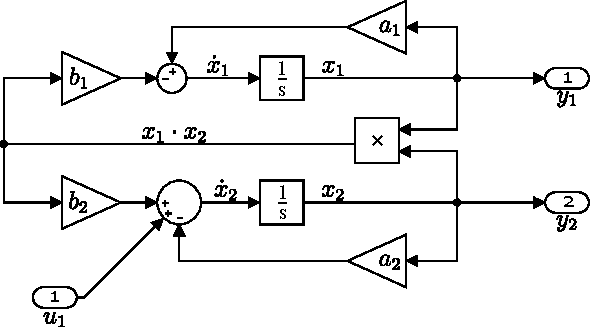
\includegraphics[width=\columnwidth]{images/ZRD_beispiel_blockdiagramm.pdf}
\end{minipage}
\hfill
\begin{minipage}[c]{0.45\columnwidth}
    \resizebox{\columnwidth}{!}{
        \renewcommand{\arraystretch}{1.3}
        \begin{tabular}{@{}ll@{}}
            $\dot{x}_1(t) = f_1(x, u)$  & $= a_1 \cdot x_1(t)$                      \\
                                        & $\quad - b_1 \cdot x_1(t) \, x_2(t)$            \\
            $\dot{x}_2(t) = f_2(x, u)$  & $= -a_2 \cdot x_2(t)$                     \\
                                        & $\quad + b_2 \cdot x_1(t) \, x_2(t) + u_1(t)$   \\
            $y_1(t) = g_1(x, u)$        & $= x_1(t)$                                \\
            $y_2(t) = g_2(x, u)$        & $= x_2(t)$
        \end{tabular}
        \renewcommand{\arraystretch}{1}
    }
\end{minipage}



\subsection{Blockdiagramm aus ZRD / Gleichung}

%NOTE: Nicht im Skirpt, kurz in V3 von Kottmann erwähnt

\begin{itemize}
    \item Auflösen nach höchster Ableitung
    \item Kette von Integratoren aufzeichnen
    \item Signale nach Integratoren wie benötigt abgreifen und Gleichung 'zusammenbauen'
\end{itemize}


\subsection{Aggregation von Teilsystemen}{172-174}
\label{Aggregation von Teilsystemen}

\textbf{Hinweis:} Grossbuchstaben und fett gedrucktes sind Matritzen


\begin{minipage}[t]{0.52\columnwidth}
    \subsubsection{Serieschaltung}

    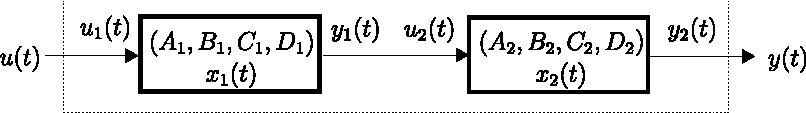
\includegraphics[width=\columnwidth]{images/ZRD_serieschaltung.pdf}
    $$
    \overbrace{ \begin{bmatrix} \dot{x}_1 \\ \dot{x}_2 \end{bmatrix}}^{\dot{x}}
    =
    \overbrace{\begin{bmatrix} A_1 & 0 \\ B_2 \cdot C_1 & A_2 \end{bmatrix} }^{\bm{A}}
    \cdot
    \overbrace{ \begin{bmatrix} x_1 \\ x_2 \end{bmatrix} }^{x}
    +
    \overbrace{ \begin{bmatrix} B_1 \\ B_2 \cdot D_1 \end{bmatrix} }^{\bm{B}} \cdot u
    $$
    $$
    y =
    \underbrace{ \begin{bmatrix} D_2 \cdot C_1 & C_2 \end{bmatrix}}_{\bm{C}}
    \cdot
    \underbrace{ \begin{bmatrix} x_1 \\ x_2 \end{bmatrix} }_{x}
    +
    \underbrace{D_2 \cdot D_1}_{\bm{D}} \cdot u
    $$
\end{minipage}
\hfill
\begin{minipage}[t]{0.45\columnwidth}
    \subsubsection{Parallelschaltung}

    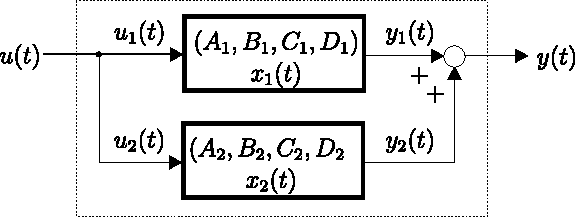
\includegraphics[width=\columnwidth]{images/ZRD_parallelschaltung.pdf}
    $$
    \overbrace{ \begin{bmatrix} \dot{x}_1 \\ \dot{x}_2 \end{bmatrix} }^{\dot{x}}
    =
    \overbrace{ \begin{bmatrix} A_1 & 0 \\ 0 & A_2 \end{bmatrix}}^{\bm{A}}
    \cdot 
    \overbrace{ \begin{bmatrix} x_1 \\ x_2 \end{bmatrix} }^{x}
    +
    \overbrace{ \begin{bmatrix} B_1 \\ B_2 \end{bmatrix} }^{\bm{B}} \cdot u
    $$
    $$
    y =
    \underbrace{ \begin{bmatrix} C_1 & C_2 \end{bmatrix} }_{\bm{C}}
    \cdot
    \underbrace{ \begin{bmatrix} x_1 \\ x_2 \end{bmatrix} }_{x}
    +
    \underbrace{(D_2 + D_1)}_{\bm{D}} \cdot u
    $$
\end{minipage}



\subsubsection{Kreisschaltung}


\begin{minipage}[c]{0.55\columnwidth}
    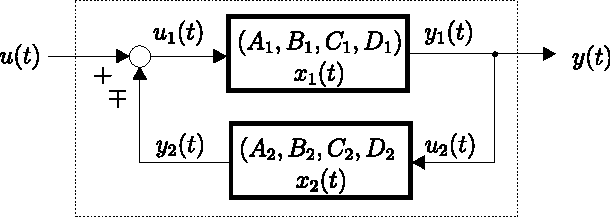
\includegraphics[width=\columnwidth]{images/ZRD_kreisschaltung.pdf}
\end{minipage}
\hfill
\begin{minipage}[c]{0.42\columnwidth}
    $$ K_1 = (I \pm D_2 D_1)^{-1} $$
    $$ K_2 = (I \pm D_1 D_2)^{-1} $$

    \begin{center}
        SISO-Systeme: $K_1 = K_2$
    \end{center}
\end{minipage}

\smallskip

$$
\overbrace{ \begin{bmatrix} \dot{x}_1 \\ \dot{x}_2 \end{bmatrix} }^{\dot{x}}
=
\overbrace{
\begin{bmatrix}
    A_1 \mp B_1 K_1 D_2 C_1 & \mp B_1 K_1 C_2           \\
    B_2 K_2 C_1             & A_2 \mp B_2 K_2 D_1 C_2
\end{bmatrix}}^{\bm{A}}
\cdot 
\overbrace{ \begin{bmatrix} x_1 \\ x_2 \end{bmatrix} }^{x}
+
\overbrace{
\begin{bmatrix} B_1 K_1 \\ B_2 K_2 D_1 \end{bmatrix} }^{\bm{B}} u
$$
$$
y =
\underbrace{ \begin{bmatrix} K_2 C_1 & \mp K_2 D_1 C_2 \end{bmatrix} }_{\bm{C}}
\cdot
\underbrace{ \begin{bmatrix} x_1 \\ x_2 \end{bmatrix} }_{x}
+
\underbrace{K_2 D_1}_{\bm{D}} \cdot u
$$

\columnbreak


\subsection{Ähnlichkeitstransformation}{175}
\label{Ähnlichkeitstransformation}


Bei der Ähnlichkeitstransformation wird eine ZRD in eine andere ZRD transformiert,
welche \textbf{dasselbe I/O-Verhalten}, aber einen \textbf{anderen internen Zustandsvektor} hat. \\
Die Ähnlichkeitstransformation wird verwendet, um ein System in eine 'besser geeignete' Form zu bringen.

\vspace{-0.2cm}

\begin{minipage}[c]{0.3\columnwidth}
    $$ \dot{x}(t) =\bm{A} \cdot x(t) + \bm{B} \cdot u(t) $$
    $$ y(t) =\bm{C} \cdot x(t) + \bm{D} \cdot u(t) $$
\end{minipage}
\hfill
\begin{minipage}[c]{0.38\columnwidth}
    $$ \underrightarrow{\text{Ähnlichkeitstransformation}} $$
\end{minipage}
\hfill
\begin{minipage}[c]{0.3\columnwidth}
    $$ \dot{\tilde{x}}(t) =\bm{\tilde{A}} \cdot \tilde{x}(t) + \bm{\tilde{B}} \cdot u(t) $$
    $$ y(t) =\bm{\tilde{C}} \cdot \tilde{x}(t) + \bm{\tilde{D}} \cdot u(t) $$
\end{minipage}

\medskip

Wenn der Zustand $x(t)$ mit einer \textbf{regulären konstanten Matrix} $\bm{P}$ multipiziert wird, ergibt sich der neue 
Zustand $\tilde{x}(t)$.
Die Umrechnungen (Ähnlichkeitstransformation) der ZRD erfolgt allgemein mittels.
$$ \boxed{ \tilde{x} = \bm{P} x \qquad  \bm{\tilde{A}} = \bm{P A P^{-1}} \qquad \bm{\tilde{B}} = \bm{P B} \qquad \bm{\tilde{C}} = \bm{C P^{-1}} \qquad \bm{\tilde{D}} = \bm{D} } $$


\subsubsection{Eigenschaften der Ähnlichkeitstransformation}

\begin{outline}
    \1 Direkte I/O-Kopplung ($\bm{\tilde{D}} = \bm{D}$) bleibt wegen gleichem I/O-Verhalten unverändert
    \1 Ändert Eigenwerte der Matix \textbf{nicht}
    \1 Ändert \textbf{nichts} an Steuerbarkeit, Beobachtbarkeit und Minimalität eines Systems
    \1 Um z.B. in einer Simulation die korrekten Signalverläufe zu berechnen, muss eine Anfangsbedingung mittransformiert werden: $\tilde{x}(0) = \bm{P} \cdot x(0)$
    \1 Wird ein System mit $\bm{P_1} = \bm{P}$ transformiert und das resultierende System mit $\bm{P_2} = \bm{P^{-1}}$ rücktransformiert, so ergibt isch wieder das ursprüngliche System
\end{outline}


\example{Zustandsvariablen in ZRD tauschen}

\begin{minipage}[c]{0.48\columnwidth}
    Eine gegebene ZRD mit Zustandsvektor $x$ soll mit Zustandsvektor $\tilde{x}$ ausgedrückt werden.
    Dafür wird die Transformationsmatrix $\bm{P}$ benötigt.
\end{minipage}
\hfill
\begin{minipage}[c]{0.48\columnwidth}
    $$ \text{ \textrightarrow } \quad \tilde{x} = \begin{bmatrix} \tilde{x}_1 \\ \tilde{x}_2 \end{bmatrix} = \begin{bmatrix} x_2 \\ x_1 \end{bmatrix}
    = \underbrace{ \begin{bmatrix} 0 & 1 \\ 1 & 0 \end{bmatrix} }_{ \bm{P} } \cdot \underbrace{ \begin{bmatrix} x_1 \\ x_2 \end{bmatrix} }_{ x } $$
\end{minipage}
%-----------------------------------------------------------------------------------------------------------------------------------
\para{Vertauschen von Zuständen}

Für

\[
\tilde x=
\begin{bmatrix}
x_2\\
x_1
\end{bmatrix}
\]

gilt

\[
P=
\begin{bmatrix}
0&1\\
1&0
\end{bmatrix}
\]

und

\[
\tilde A=PAP^{-1},
\qquad
\tilde B=PB,
\qquad
\tilde C=CP^{-1}
\]
%-----------------------------------------------------------------------------------------------------------------------------------